\documentclass[a4paper,12pt]{ctexart}
\usepackage{amsmath}
\usepackage{amsfonts}
\usepackage{float}
\usepackage{enumerate}
\usepackage{graphicx}
\usepackage{booktabs}
\usepackage{float}
\usepackage{hyperref}
\renewcommand{\listfigurename}{图表目录}
\setcounter{secnumdepth}{0}
\title{Atlassian:乘云而起,协作为先}
\author{董晨阳}
\date{\today}
\begin{document}
\maketitle
\begin{abstract}
    \textbf{Atlassian是全球领先的软件开发协作云平台}。其业务线包括敏捷开发与DevOps、工作协同、IT服务管理,拳头产品包括Jira Software、Confluence、JSM等,覆盖软件开发全流程,链接需求与开发和业务团队。公司轻营销、重研发,non-GAAP净利持续为正。

    \textbf{Atlassian的成功既包括公司的奋斗,也包括历史的进程}。Atlassian抓住了软件工程领域敏捷开发和DevOps两次革命的先机,率先上云并受疫情远程办公需求催化。公司专注于团队协作领域,从开发团队协作逐步扩展到全公司的知识协作与IT服务协作,通过免费与集成吸引潜在用户群,并通过飞轮效应使得免费用户转化为付费用户,并向周围人推荐吸引更多免费用户。

    \textbf{当前Atlassian短期增长承压,长期看增长逻辑并未改变}。受宏观逆风和竞争加剧等影响,Atlassian用户增长速度和免费用户转化率有所下滑,并且公司逆周期扩张战略可能导致短期盈利压力。但长期看公司基本面并未有重大改变,关注长期竞争格局演变与新产品渗透转化情况。

    \textbf{风险提示}:宏观逆风超预期、免费用户转化率不足、企业上云进度不及预期、竞争不及对手、新产品研发渗透不及预期、网络安全风险
\end{abstract}
\clearpage
\tableofcontents
\listoffigures
\clearpage
\section{Atlassian:团队合作的力量}

\textbf{Atlassian为全球领先的项目管理、内容协同SaaS厂商}。Atlassian位于澳大利亚,提供面向企业业务流程的协同办公产品,多年位居Gartner魔力象限的领导者象限。Atlassian主要面向软件开发者,也向企业技术人员、知识工作者等群体扩展。财富500强中的大多数以及全球超过240,000家各种规模的公司都依赖Atlassian的解决方案来帮助他们的团队更好地合作并按时交付高质量的结果。在,包括Jira软件、Confluence、Jira服务管理、Trello、BitBucket和Jira Align等。
\begin{figure}[H]
    \centering
    \begin{minipage}{0.38\linewidth}
        \caption{Atlassian位于魔力象限的领导者}
        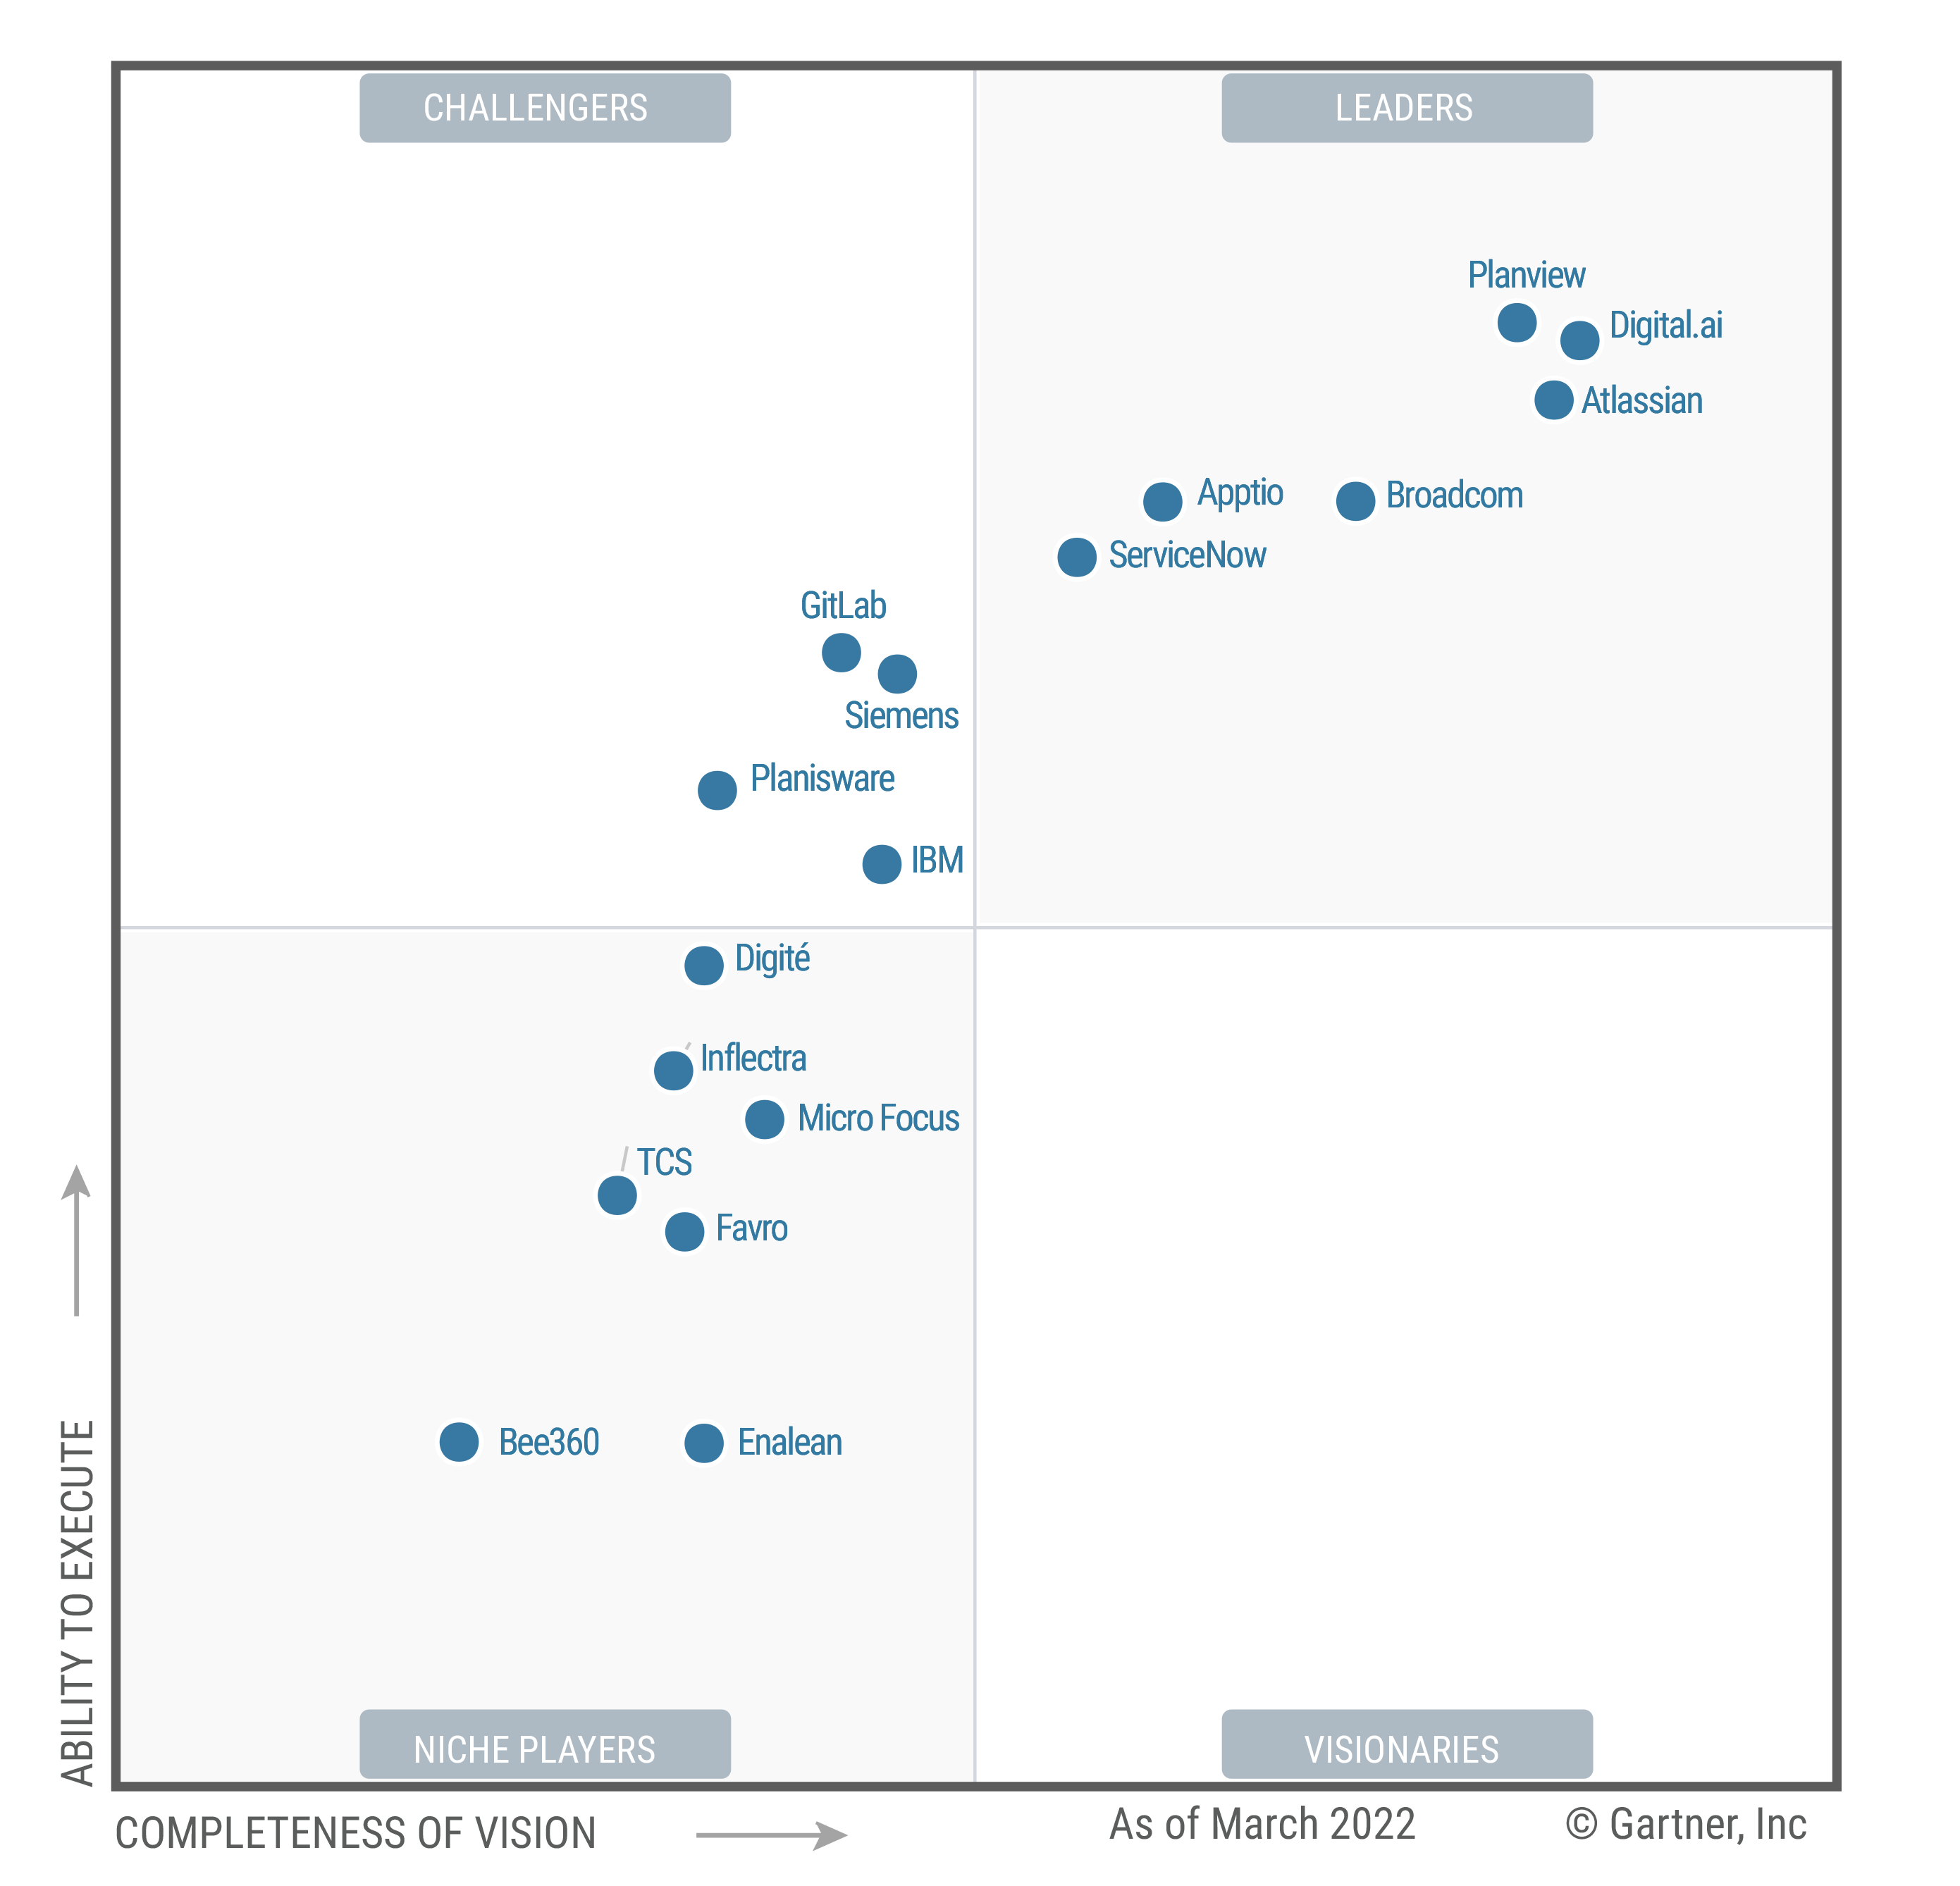
\includegraphics[width=\linewidth]{img/gartner.png}
        \footnotesize{资料来源:Gartner}
    \end{minipage}
    \begin{minipage}{0.58\linewidth}
        \caption{Atlassian用户数}
        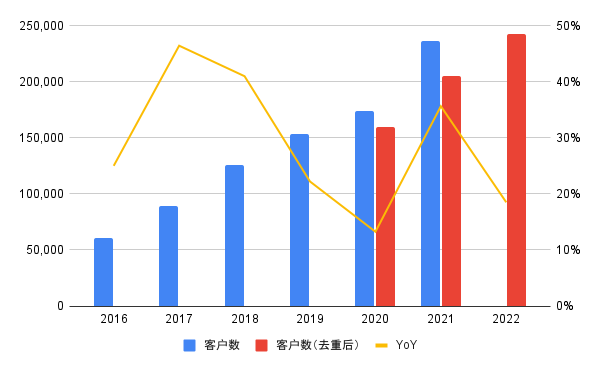
\includegraphics[width=\linewidth]{img/customers.png}
        \footnotesize{资料来源:公司公告。注:1Q22更换统计口径,不同产品的用户数去重}
    \end{minipage}
\end{figure}

\textbf{Jira和Confluence是Atlassian的核心产品,满足软件开发行业敏捷开发等需求}。Atlassian公司成立于2002年,在成立两年内发布了拳头产品Jira和Confluence,并在2010年将产品迭代上云,于2015年上市。Atlassian还通过不断并购扩大产品矩阵,如项目管理软件Trello、代码托管网站Bitbucket、Git客户端SourceTree等。这些软件都与Jira和Confluence高度集成,形成丰富的产品生态。
\begin{figure}[H]
    \caption{Atlassian公司历史}
    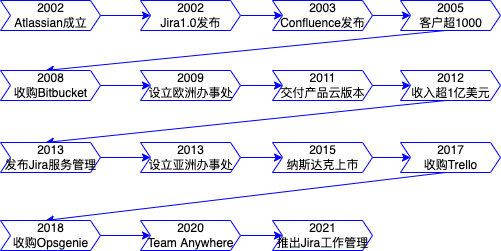
\includegraphics[width=\linewidth]{img/timeline.drawio.png}
    \footnotesize{资料来源:公司公告}
\end{figure}

\subsection{Atlassian的财务水平}

\textbf{Atlassian 的收入主要来自订阅收入、永久许可、维修收入和其他来源}。其中:
\begin{enumerate}
    \item 订阅是 Atlassian 收入的主要来源,占比逐年提高,1Q23占总收入的 80\%。订阅收入主要由活跃许可证的数量和大小、产品类型和许可证的价格驱动,预计未来受益于云计算进一步普及仍将持续增加。
    \item 永久许可证收入包括从向新客户销售许可证、增加现有客户中的用户数量和向现有客户增加许可证中确认的收入。2022年Atlassian取消了永久许可证业务,鼓励用户转向云订阅。
    \item 维护收入是指为永久许可产品向客户支持所获得的费用,但受永久许可证不再签发影响有所萎缩。
    \item 其他收入包括在 Atlassian Marketplace销售第三方应用程序和培训服务的费用。Atlassian Marketplace类似App Store,在第三方销售收入中抽成比例为15-25\%。这部分收入随Atlassian生态的逐步完善吸引更多第三方应用开发者,增长也非常迅速,但体量较小。
\end{enumerate}
\begin{figure}[H]
    \caption{Atlassian分业务收入(万美元)}
    \begin{center}
        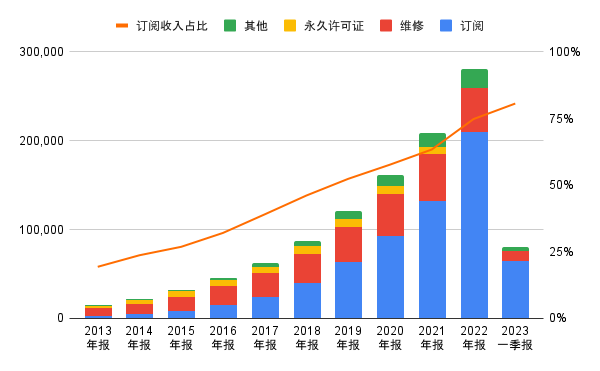
\includegraphics[width=\linewidth]{img/revenue.png}
    \end{center}
    \footnotesize{资料来源:同花顺iFind}
\end{figure}

\textbf{费用上,Atlassian轻营销、重研发}。一般的SaaS和软件厂商由于大量的营销费用呈现出高毛利、低净利的情况。Atlassian采用直销的方式降低营销成本,并且拳头产品的口碑非常好,一度不需要销售人员。Atlassian 销售费用率始终低于研发费用率,销售费用率常年在 20\%上下浮动(正常的 SAAS 企业销售费用率在40\%-60\%,个别企业甚至在 80\%左右)。此外Atlassian重研发,不断研发新功能以贴合软件行业的快速发展。近期Atlassian出于逆周期扩张的战略S\&M、G\&A费用率均有所增加。
\begin{figure}[H]
    \caption{Atlassian费用水平(万美元)}
    \begin{center}
        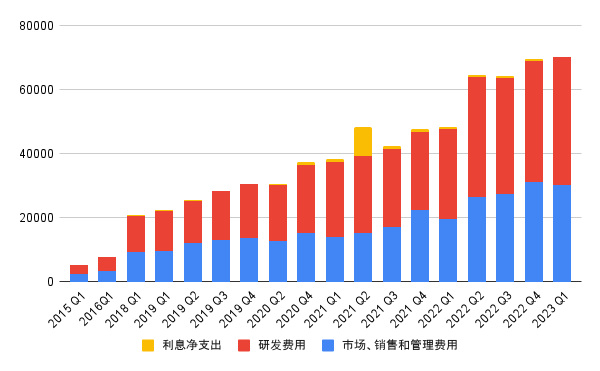
\includegraphics[width=0.8\linewidth]{img/cost.png}
    \end{center}
    \footnotesize{资料来源:同花顺iFind}
\end{figure}

\textbf{Atlassian保持长期盈利,non-GAAP净利持续为正}。Atlassian在未上市时便保持了长期的盈利,上市后营业利润率保持增长趋势,但在2022年出于公司战略营业利润率有所下滑。
\begin{figure}[H]
    \caption{non-GAAP口径下Atlassian财务状况}
    \begin{center}
        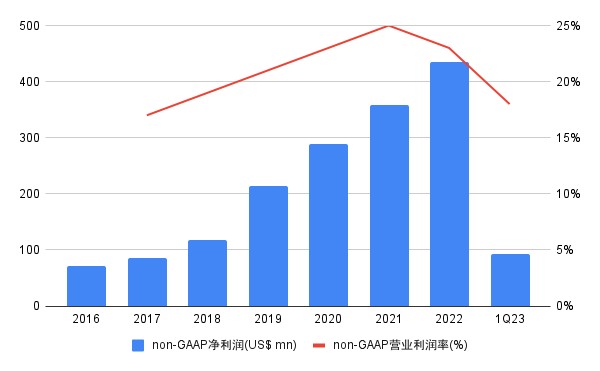
\includegraphics[width=0.7\linewidth]{img/non-GAAP.png}
    \end{center}
    \footnotesize{资料来源:公司公告}
\end{figure}

\subsection{Atlassian的产品线}
Atlassian的产品线主要有以下四条:用于团队计划和项目管理的 Jira系列等、用于团队内容创建和协作的 Confluence和Trello等、用于团队编写代码和管理审查的 Bitbucket和SourceTree等、以及用于身份与安全的Atlassian Access等。

\textbf{Jira在敏捷开发时代为组织提供了工作流}。Jira 是一个复杂而灵活的工作流管理系统,帮助团队计划组织、跟踪Bug和管理项目。Jira Software 专为软件团队中的每位成员构建,可供其用于规划、跟踪和发布卓越的软件,具有规划、跟踪、发布、报告和自动化五大用途。Jira Service连接开发、IT 运营和业务团队,快速响应需求变更,提升开发敏捷度。Atlassian旗下的另一款软件Opsgene则集中管理警报,在业务逻辑发生问题时及时通知给正确的人。此外Jira也集成到Atlassian体系外的常用办公软件,如Slack等。
\begin{table}[H]
    \caption{Jira Software 五大用途}
    \begin{tabular}{ll}
        \toprule
        用途  & 内容                             \\
        \midrule
        规划  & 通过用户故事、事务和任务,将宏大计划分解为易于管理的部分   \\
        跟踪  & 追踪bug与需求,排定整个环境中团队工作的优先次序并进行讨论 \\
        发布  & 加速交付,同时保证自己所拥有的信息保持最新          \\
        报告  & 根据直观的实时数据,在整体环境下提升团队绩效         \\
        自动化 & 通过无代码自动化功能,节省时间、保持专注、顺畅工作流     \\
        \bottomrule
    \end{tabular}
    \footnotesize{资料来源:Atlassian}
\end{table}

\textbf{Confluence作为企业内部的知识wiki,实现企业内部的知识共享}。Confluence 是一个社会性的、灵活的内容协作平台,用于创建、共享、组织和讨论项目。不同于一般的协作文档,Confluence针对技术团队提供了大量的规范模版,并支持富媒体编辑,满足技术文档中的UML类图、Visio图、流程图的需求;文档中还可以内嵌评审流程,不止于仅仅@某人,关联研发过程。通过软件开发者中的盛誉,Confluence也向企业技术人员、知识工作者等群体破圈传播。
\begin{figure}[H]
    \caption{Confluence可以与Jira集成}
    \begin{center}
        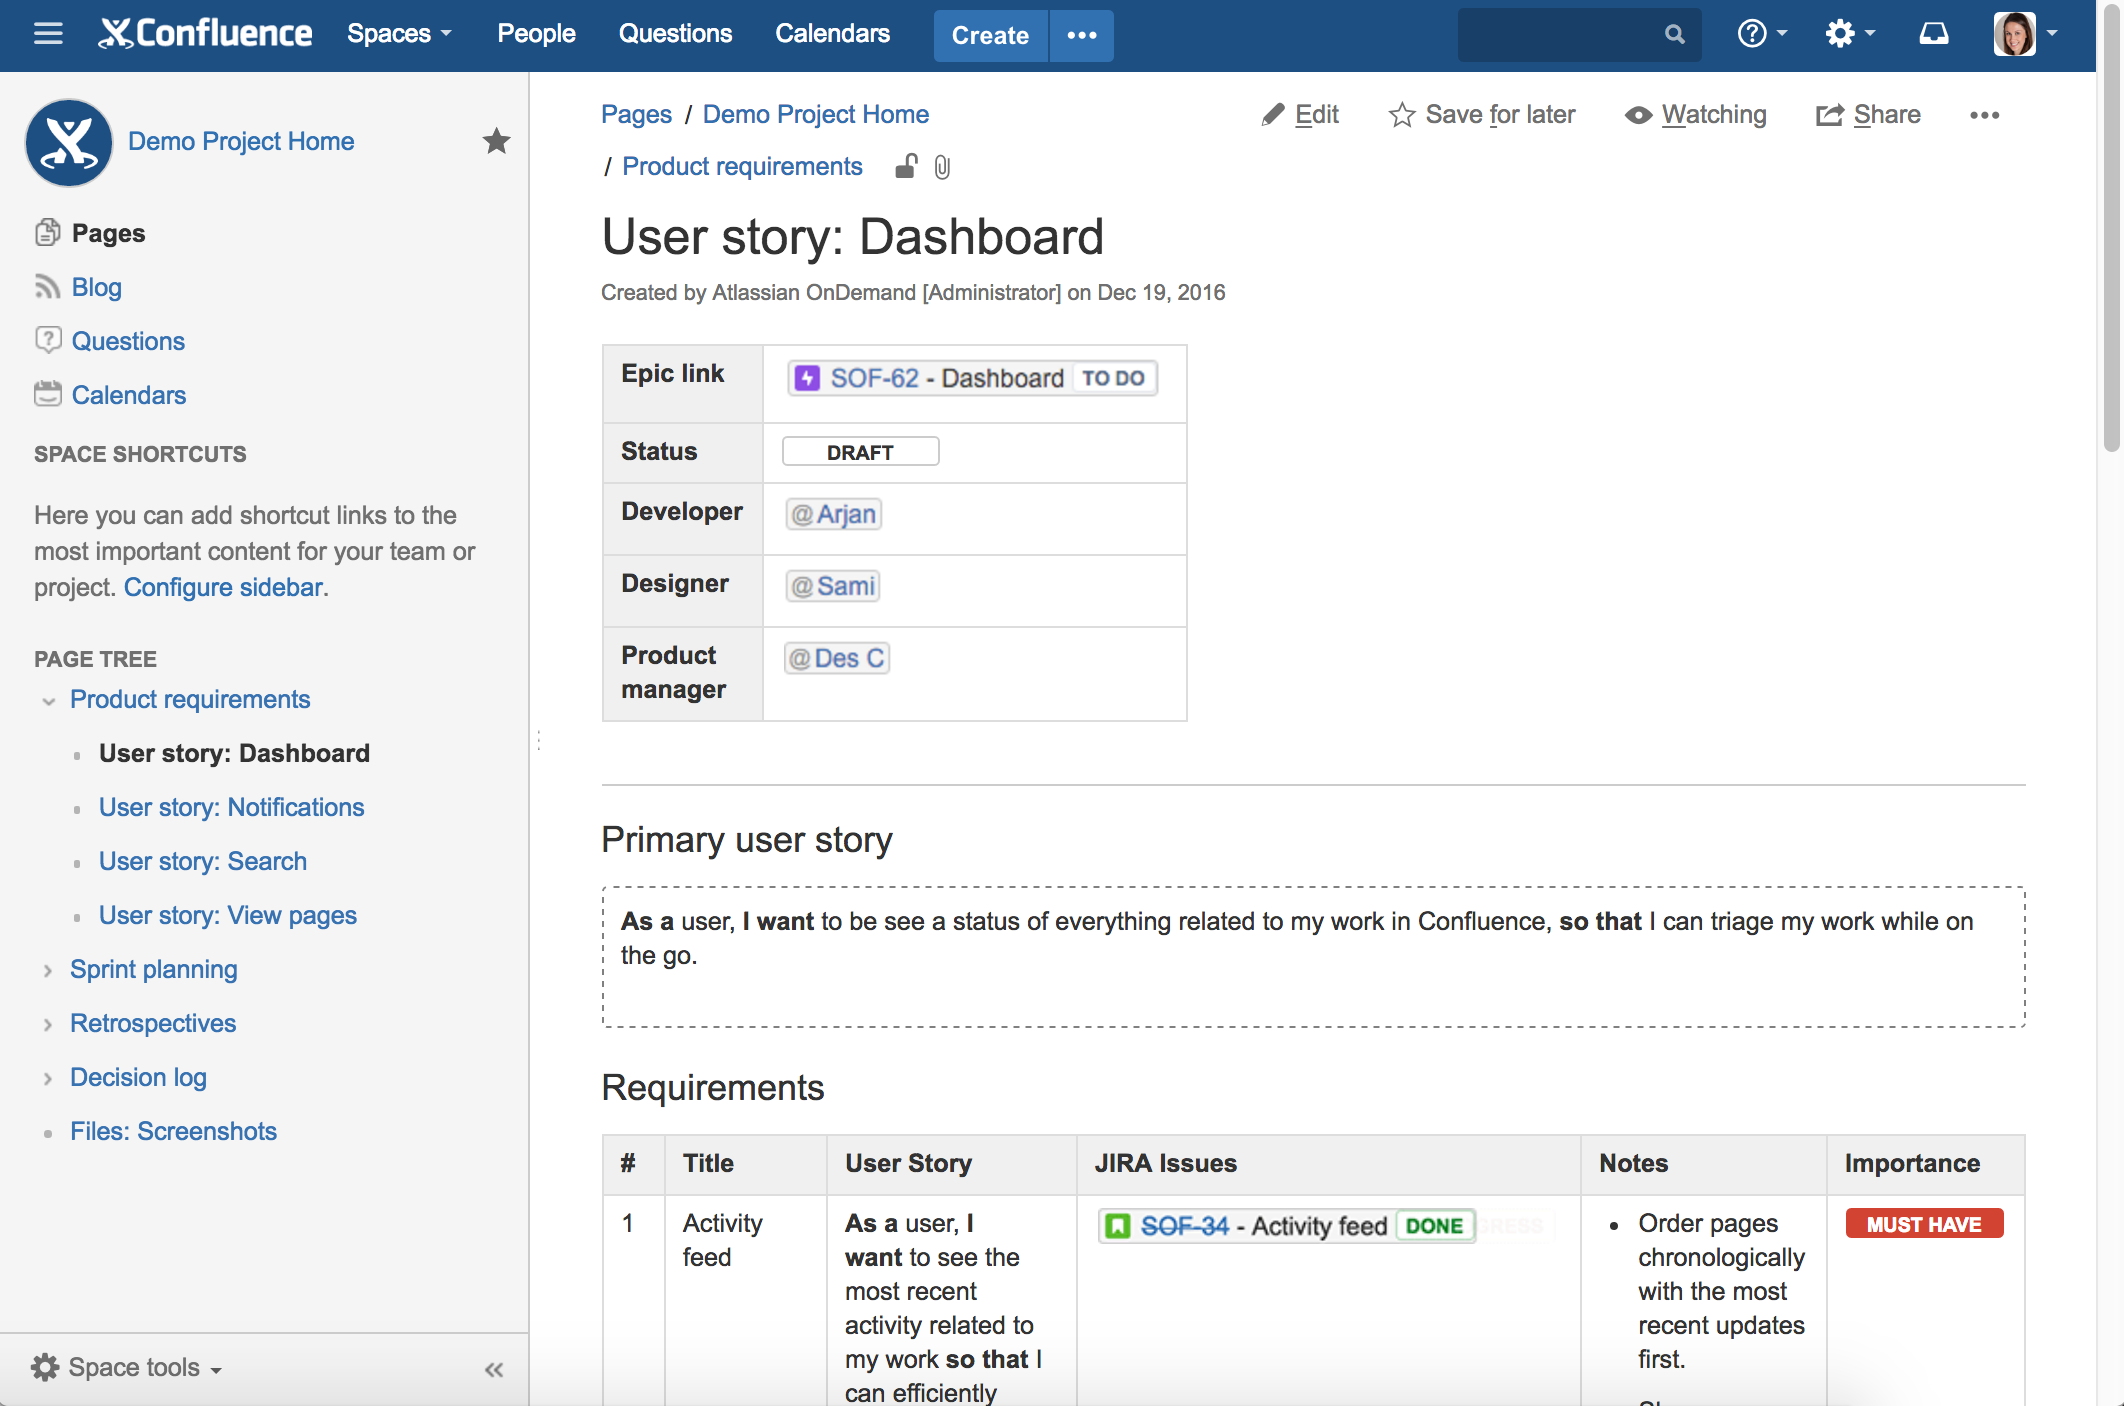
\includegraphics[width=0.8\linewidth]{img/Using+Confluence+with+JIRA.png}
    \end{center}
    \footnotesize{资料来源:Atlassian Documentation}
\end{figure}

\textbf{Trello专注于更通用的任务管理}。Jira所包含的任务管理主要是和敏捷开发相关的,以开发一个软件产品为目标。Trello则提供了更通用的看板,提供了任务进度等要素,帮助团队对任务进行计划。
\begin{figure}[H]
    \begin{minipage}{0.48\linewidth}
        \caption{Jira任务管理基于产品目标}
        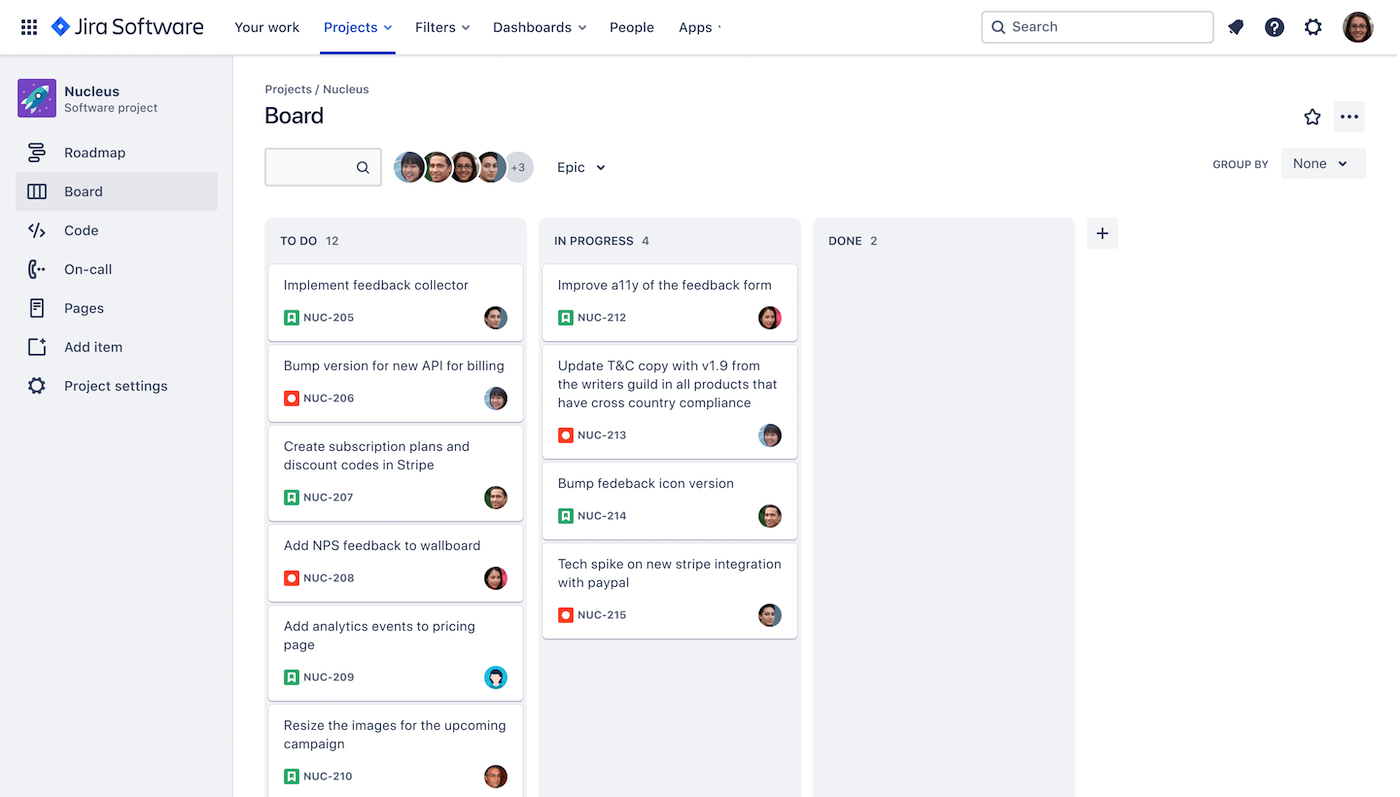
\includegraphics[width=\linewidth]{img/jira.png}
    \end{minipage}
    \begin{minipage}{0.48\linewidth}
        \caption{Trello任务管理更为通用}
        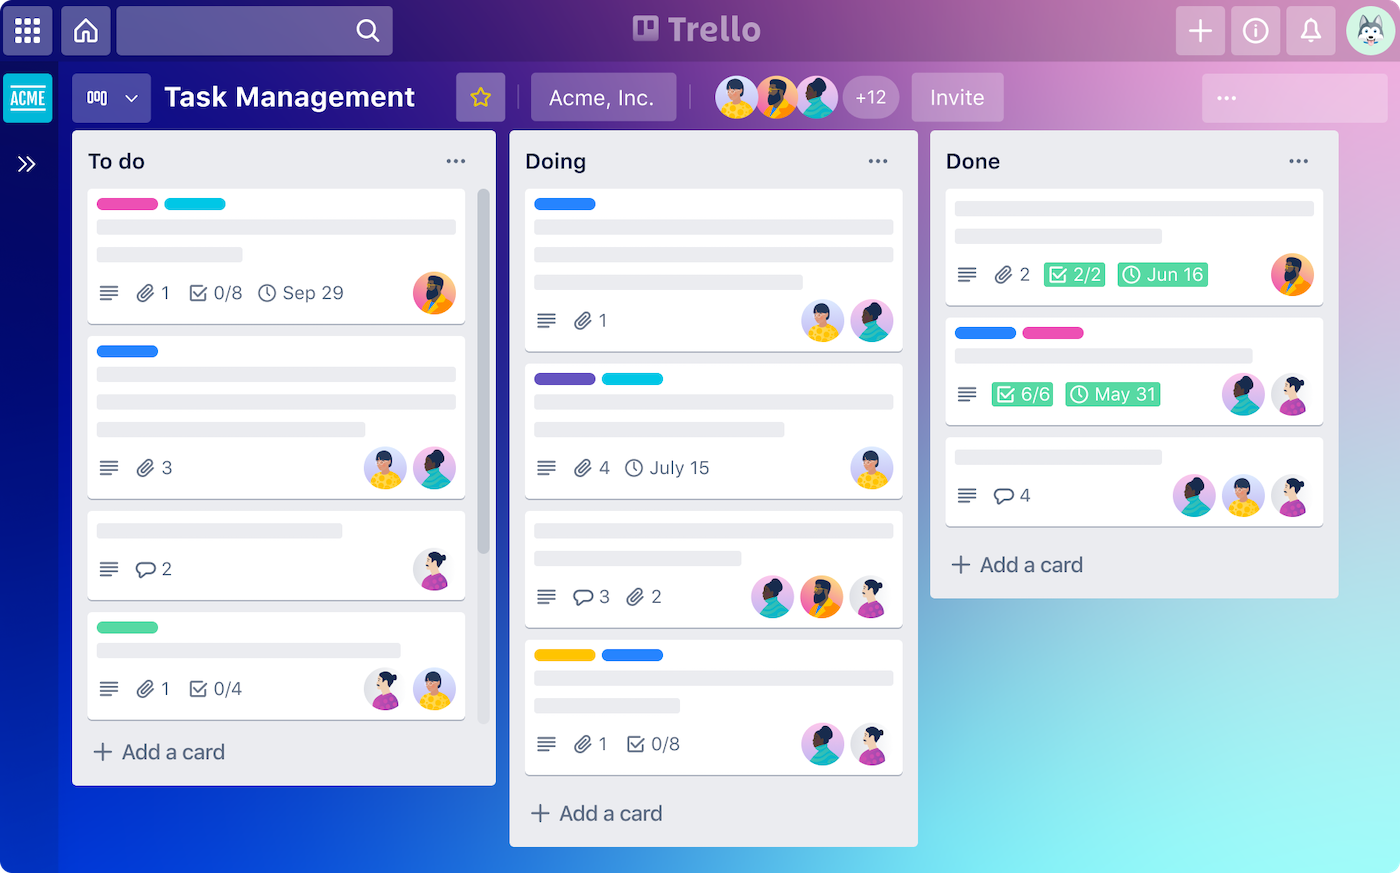
\includegraphics[width=\linewidth]{img/Trello.png}
    \end{minipage}
    \footnotesize{资料来源:technologyadvice}
\end{figure}

\textbf{Bitbucket类似GitHub与GitLab,对Jira有更强的集成}。BitBucket 是 2008 年创建的源代码托管网站,采用 Mercurial 和 Git 作为分布式版本控制系统,同时提供免费账户和商业计划。2010 年被 Atlassian 收购,与 Atlassian 的其他服务(Jira、SourceTree、Bamboo、Crucible等)高度集成,其主要市场是大型企业。

Atlassian Access等简化了 Okta 和 SSO 的登录流程,可将用户的 Atlassian 云产品与身份提供商连接起来。

\section{现状:产品力强大,链接企业内外}

\subsection{财务状况:订阅收入为主,non-GAAP稳定盈利}

\textbf{Atlassian 的收入主要来自订阅收入、永久许可、维修收入和其他来源}。其中:
\begin{enumerate}
    \item 订阅是 Atlassian 收入的主要来源,占比逐年提高,1Q23占总收入的 80\%。订阅收入主要由活跃许可证的数量和大小、产品类型和许可证的价格驱动,预计未来受益于云计算进一步普及仍将持续增加。
    \item 永久许可证收入包括从向新客户销售许可证、增加现有客户中的用户数量和向现有客户增加许可证中确认的收入。2021年Atlassian取消了永久许可证业务,鼓励用户转向云订阅。
    \item 维护收入是指为永久许可产品向客户支持所获得的费用,但受永久许可证不再签发影响有所萎缩。
    \item 其他收入包括在 Atlassian Marketplace销售第三方应用程序和培训服务的费用。Atlassian Marketplace类似App Store,在第三方销售收入中抽成比例为15-25\%。这部分收入随Atlassian生态的逐步完善吸引更多第三方应用开发者,增长也非常迅速,但体量较小。
\end{enumerate}
\begin{figure}[H]
    \caption{Atlassian分业务收入(万美元)}
    \begin{center}
        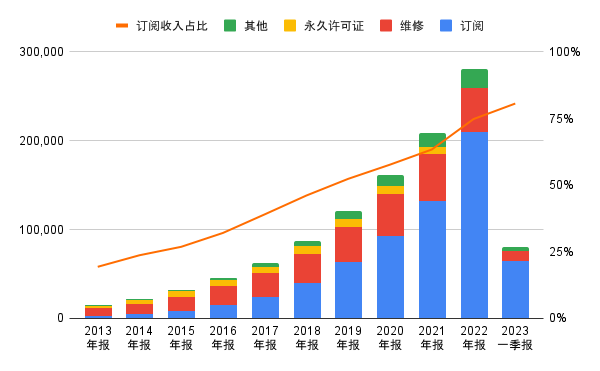
\includegraphics[width=\linewidth]{img/revenue.png}
    \end{center}
    \footnotesize{资料来源:同花顺iFind}
\end{figure}

\textbf{费用上,Atlassian轻营销、重研发}。一般的SaaS和软件厂商由于大量的营销费用呈现出高毛利、低净利的情况。Atlassian采用直销的方式降低营销成本,并且拳头产品的口碑非常好,一度不需要销售人员。Atlassian 销售费用率始终低于研发费用率,销售费用率常年在 20\%上下浮动(正常的 SAAS 企业销售费用率在40\%-60\%,个别企业甚至在 80\%左右)。此外Atlassian重研发,研发费用率接近50\%,不断研发新功能以贴合软件行业的快速发展。近期Atlassian将挑战性的宏观经济环境视为抢占市场份额并继续投资于战略性高增长领域的机会,费用率均有所增加。

\begin{figure}[H]
    \caption{Atlassian费用水平(万美元)}
    \begin{center}
        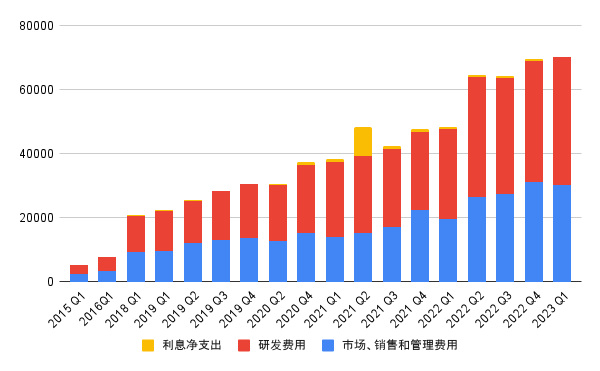
\includegraphics[width=0.9\linewidth]{img/cost.png}
    \end{center}
    \footnotesize{资料来源:同花顺iFind}
\end{figure}
\begin{figure}[H]
    \caption{同行业其他公司的销售费用率对比}
    \begin{center}
        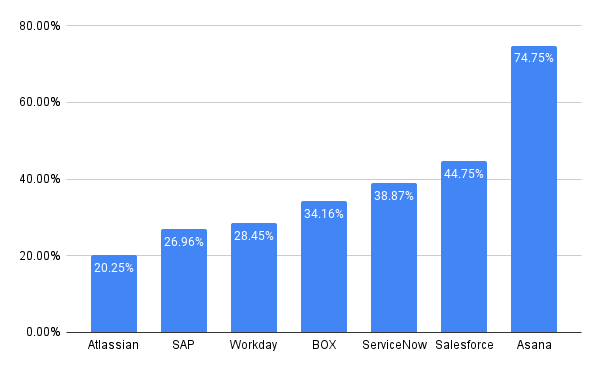
\includegraphics[width=0.9\linewidth]{img/SM.png}
    \end{center}
    \footnotesize{资料来源:同花顺iFind}
\end{figure}

\textbf{Atlassian保持长期盈利,non-GAAP净利持续为正}。Atlassian在未上市时便保持了长期的盈利,上市后营业利润率保持增长趋势,但2022年由于公司扩张战略、叠加高通胀的宏观环境,公司的营业利润率有所下滑。
\begin{figure}[H]
    \caption{non-GAAP口径下Atlassian财务状况}
    \begin{center}
        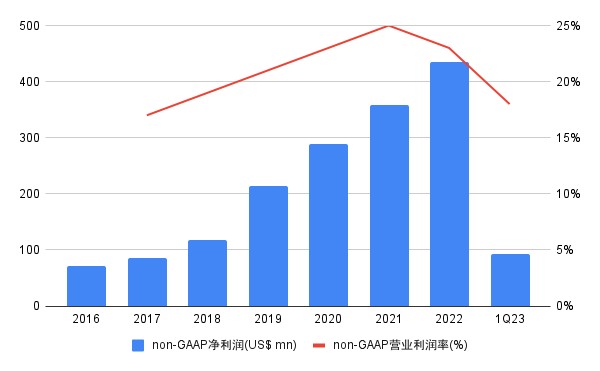
\includegraphics[width=\linewidth]{img/non-GAAP.png}
    \end{center}
    \footnotesize{资料来源:公司公告}
\end{figure}

\subsection{产品线:覆盖软件开发流程,链接需求、开发团队与业务团队}
Atlassian的产品线主要有以下几条:协助团队敏捷开发、DevOps的 Jira Software(以下简称为Jira)和Bitbucket等、用于工作协同的 Confluence和Trello等、用于IT服务的Jira Service Management。Atlassian新推出了Atlassian Together订阅套餐,包括了Tello、Confluence、Jira产品等。

\textbf{Jira等一系列应用在敏捷开发时代为软件开发组织提供了工作流}。互联网行业的快速发展使得敏捷开发快速响应需求的重要性大大提升,但组织、代码和事务的复杂度严重拖累了敏捷响应的速度。Atlassian提供了一整套全流程的敏捷开发与DevOps解决方案以对抗复杂度:核心产品Jira具有规划、跟踪、发布、报告和自动化五大用途,将事务与代码关联起来,可以规划分配大型任务,并提供了许多标准工作流辅助开发;与Jira高度集成的代码托管网站Bitbucket则覆盖了代码的编写、审查和CI/CD;Atlassian旗下的另一款软件Opsgene则集中管理警报,在业务逻辑发生问题时及时通知给正确的人,也与Jira高度集成;Statuspage则负责监控软件的日常运行。Jira自发布以来广受赞誉,以Jira为核心的软件开发全流程覆盖是Atlassian的核心竞争力之一。
\begin{figure}[H]
    \caption{Jira依旧是使用最多的敏捷开发工具}
    \begin{center}
        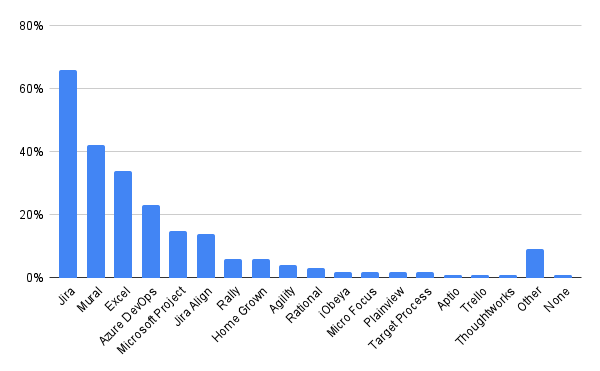
\includegraphics[width=\linewidth]{img/popularity.png}
    \end{center}
    \footnotesize{资料来源:digital.ai。注:digital.ai的Agility为Jira竞品}
\end{figure}
\begin{table}[H]
    \caption{Jira Software 五大用途}
    \begin{tabular}{ll}
        \toprule
        用途  & 内容                             \\
        \midrule
        规划  & 通过用户故事、事务和任务,将宏大计划分解为易于管理的部分   \\
        跟踪  & 追踪bug与需求,排定整个环境中团队工作的优先次序并进行讨论 \\
        发布  & 加速交付,同时保证自己所拥有的信息保持最新          \\
        报告  & 根据直观的实时数据,在整体环境下提升团队绩效         \\
        自动化 & 通过无代码自动化功能,节省时间、保持专注、顺畅工作流     \\
        \bottomrule
    \end{tabular}
    \footnotesize{资料来源:Atlassian}
\end{table}

\textbf{工作协同方面,Confluence实现企业内部的知识共享,Trello专注于通用的任务管理}。Confluence是一个社会性的、灵活的内容协作平台,用于创建、共享、组织和讨论项目。不同于一般的协作文档,Confluence针对技术团队提供了大量的规范模版,并支持富媒体编辑,满足技术文档中的UML类图、Visio图、流程图的需求;文档中还可以内嵌评审流程,不止于仅仅@某人,关联研发过程。通过软件开发者中的盛誉,Confluence也向企业技术人员、知识工作者等群体破圈传播。相较于Jira所包含的以敏捷开发一个软件产品为目标的任务管理,Trello则提供了更通用的看板,提供了任务进度等要素,帮助团队对任务进行计划。
\begin{figure}[H]
    \begin{minipage}{0.48\linewidth}
        \caption{Jira任务管理基于产品目标}
        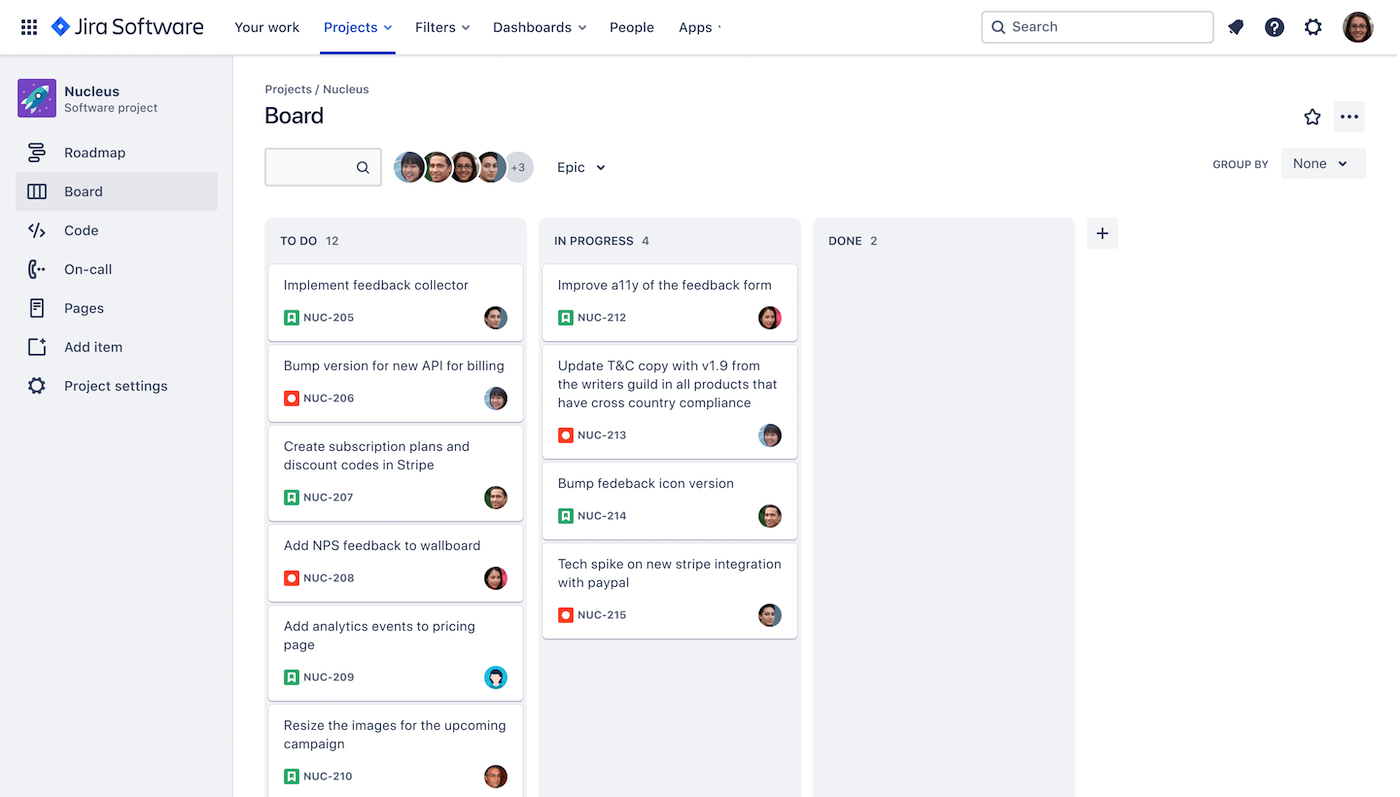
\includegraphics[width=\linewidth]{img/jira.png}
    \end{minipage}
    \begin{minipage}{0.48\linewidth}
        \caption{Trello任务管理更为通用}
        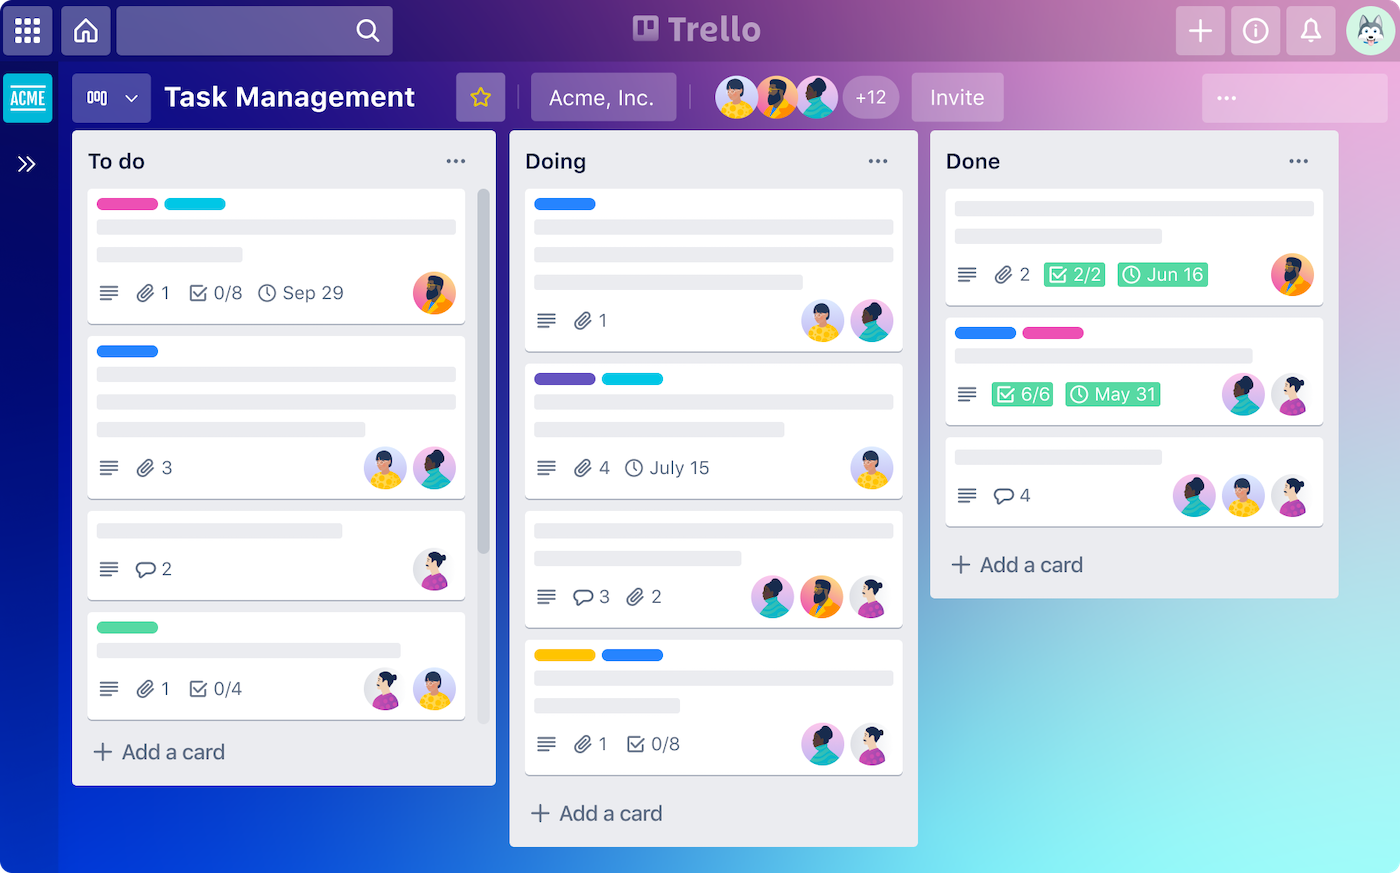
\includegraphics[width=\linewidth]{img/Trello.png}
    \end{minipage}

    \footnotesize{资料来源:technologyadvice}
\end{figure}

\textbf{IT服务管理(ITSM)方面,Jira Service Management(JSM)连接开发、IT 运营和业务团队}。企业提供技术服务的瓶颈并不只是技术层面,流程管理与人员疏失的失误可能会导致IT服务的失败,因而需要ITSM以保证IT服务质量,协作不应当局限在开发团队而是所有团队,所以Atlassian推出了JSM。JSM可以作为自助服务门户,为用户提供了一个可以寻求帮助的地方。客户需要服务时可以向JSM请求帮助,企业内部可以履行或通过ITSM移交服务请求给其他适当团队,如IT、人力、法律和财务团队等。Jira Service Management在 Jira 之上提供专业的 ITSM 功能,将开发、运营和业务团队汇聚在一起,以便他们可以及时响应业务变更并快速提供出色的服务体验,目前市占率(18.5\%)排行第二,仅次于ServiceNow(40.1\%)。
\begin{figure}[H]
    \caption{JSM功能}
    \begin{center}
        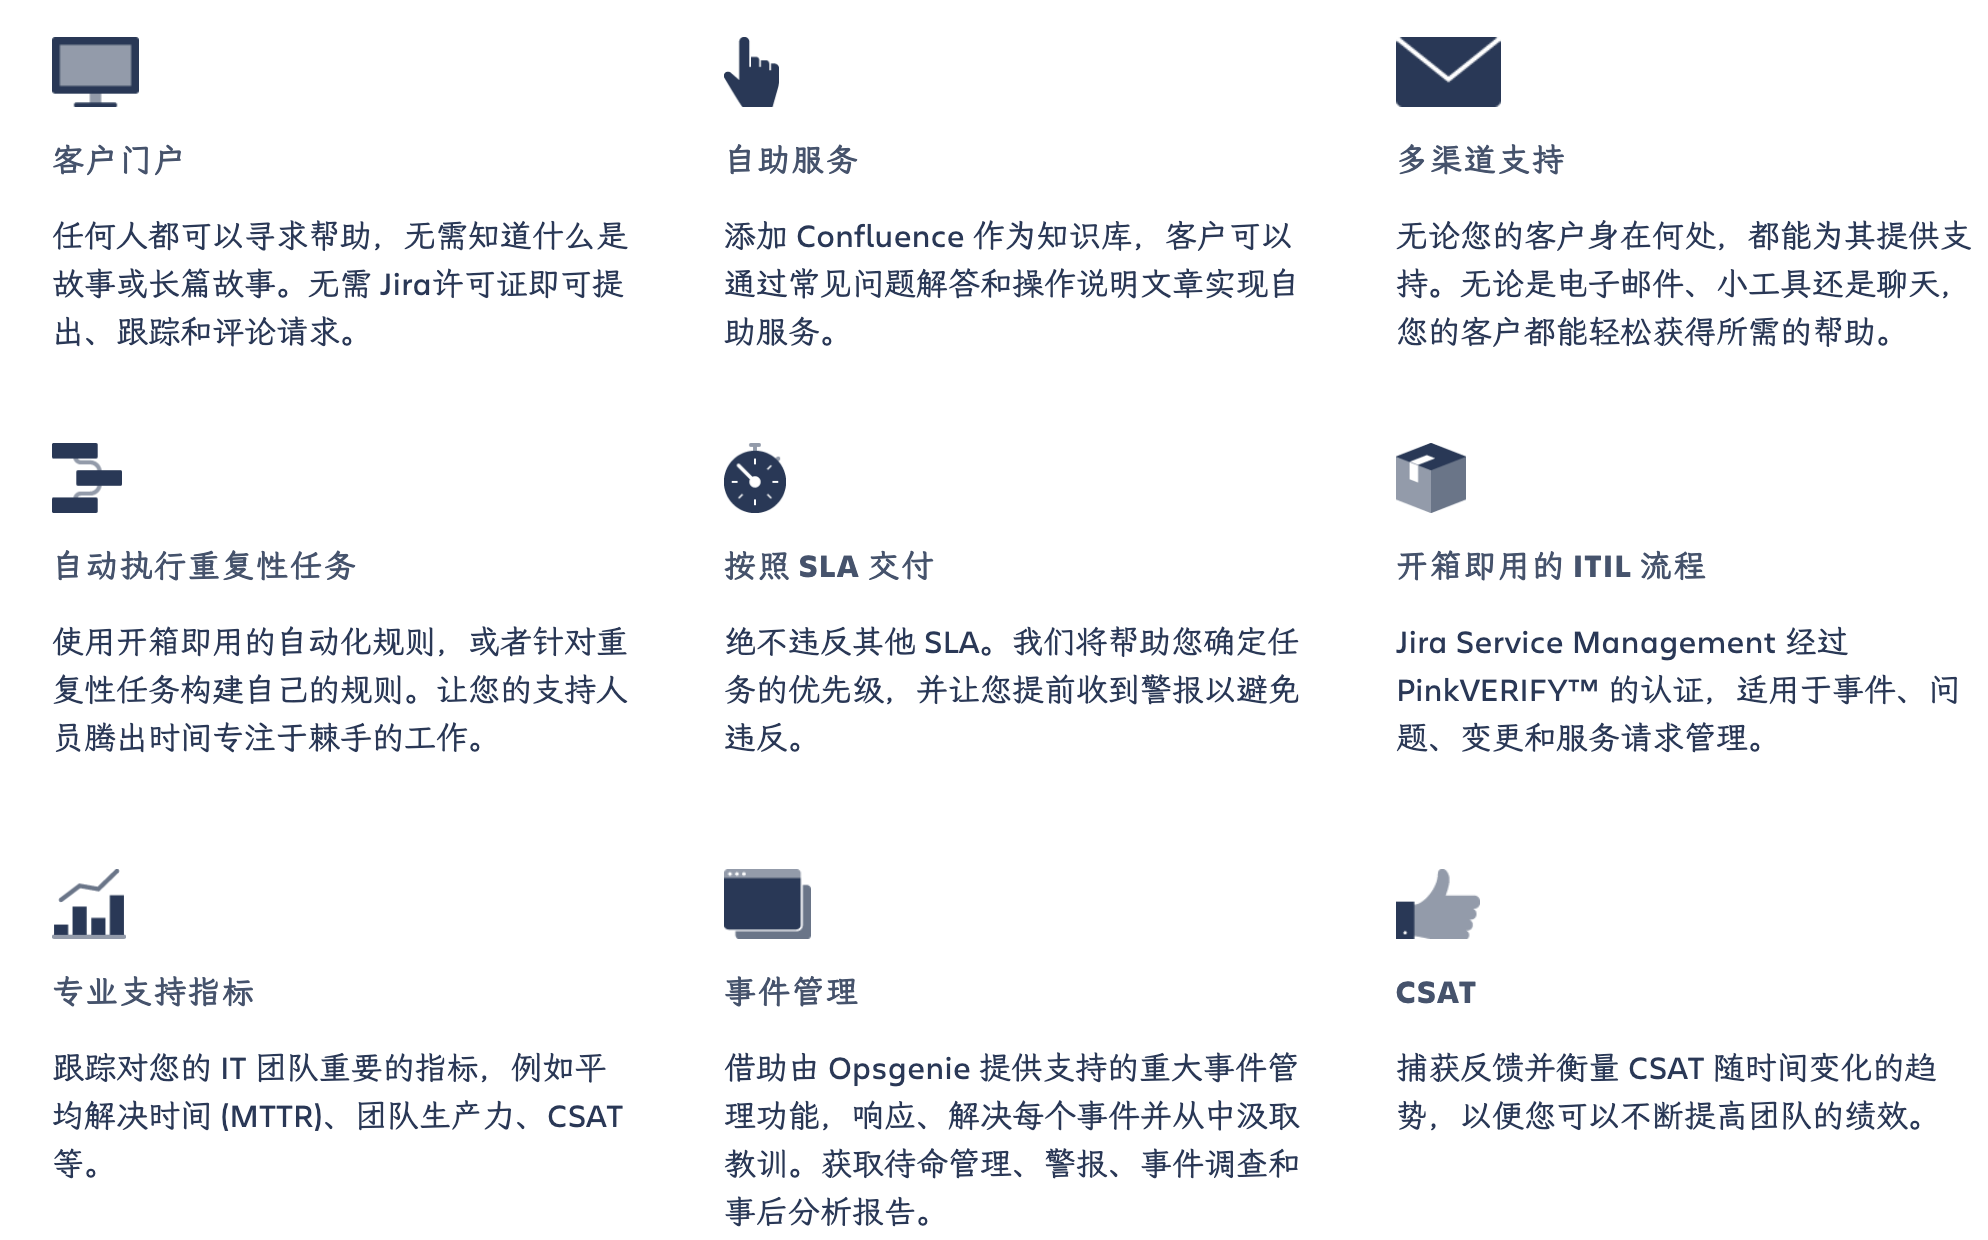
\includegraphics[width=0.9\linewidth]{img/ITSM.png}
    \end{center}
    \footnotesize{资料来源:atlassian}
\end{figure}

\subsection{行业:百舸争流,角逐激烈}

目前Atlassian在三个产品领域均有竞争对手,但市场空间相对广阔。根据\href{https://startuptalky.com/atlassian-success-story/}{startuptalky},2021 年,项目管理软件市场产生了 53.596 亿美元的销售额。到 2032 年,项目管理软件市场的收入预计将达到 204亿美元,2022 年至 2032 年的复合年增长率为 13.1\%。与之相对Atlassian年化收入仅16亿美元。且Atlassian凭借∆强大的产品力具有一定的竞争优势。

开发工具方面,据enlyft,Jira市场份额约为28.95\%。其主要竞争对手包括微软(Azure Board与GitHub Enterprise)、GitLab、IBM、Broadcom(Rally)、Asana、JetBrains(YouTrack)等。据Gartner,Jira为最受欢迎的敏捷开发工具,相较于其他产品服务更加完善、更易部署、价格相对便宜。

工作协同领域竞争较为激烈。据enlyft,文档工具领域Confluence市场份额约为2.25\%,任务管理领域Trello占统治性地位,市占率达74.1\%。Atlassian在这些方面的主要竞争对手包括微软Office、Slack、Adobe、Google Workspace、Notion等,在技术文档的细分领域Confluence凭借富媒体、易集成等具有一定的比较优势。

ITSM方面,其主要竞争对手包括ServiceNow、GoTo、微软等,JSM在ITSM市占率仅次于ServiceNow,达18.5\%。
\begin{figure}[H]
    \caption{JSM在ITSM领域市占率排第二}
    \begin{center}
        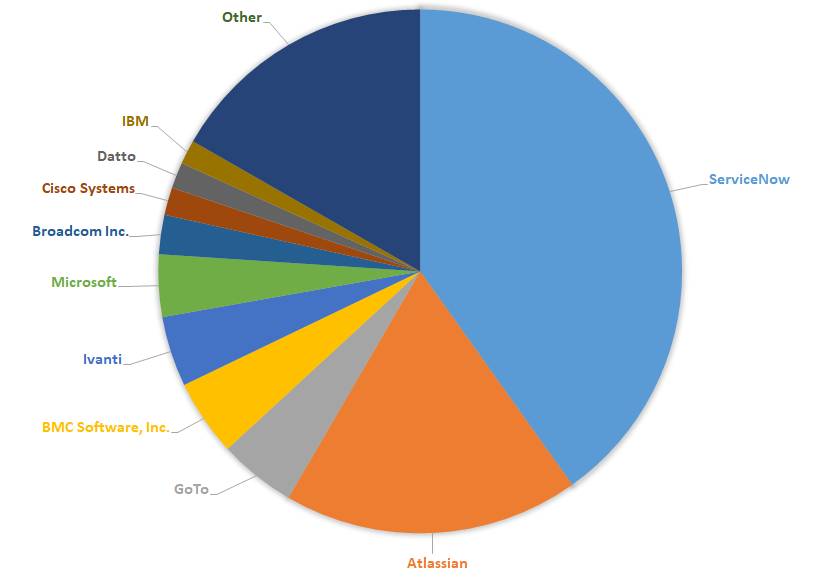
\includegraphics[width=0.9\linewidth]{img/JSM.png}
    \end{center}
    \footnotesize{资料来源:Apps Run The World}
\end{figure}

\section{增长动力:顺应时代趋势,做精团队合作}
Atlassian成长至今,增长的来源既有敏捷开发普及、全面上云的时代红利,也有公司内部持续迭代、打磨团队合作的内驱动力。
\begin{figure}[H]
    \caption{Atlassian与美股SaaS指数复盘}
    \begin{center}
        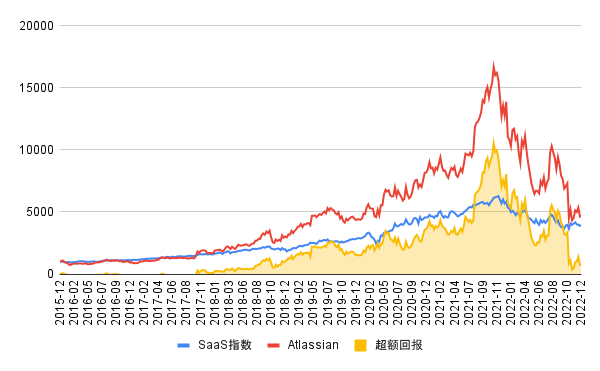
\includegraphics[width=0.9\linewidth]{img/excessreturn.png}
    \end{center}
    \footnotesize{资料来源:Wind。注:指数与股价初值归一为1000。}
\end{figure}

\subsection{时代的\texorpdfstring{$\beta$}——敏捷开发与DevOps、全面上云、疫情催化}
\textbf{软件工程经历了瀑布式开发、敏捷开发与DevOps三个阶段,Atlassian抓住了后两个阶段的时代机遇}。具体而言:
\begin{enumerate}
    \item 及时响应敏捷开发。1980年代的传统瀑布模型流程有严格的先后之分,自上而下的流程像极了瀑布的下落,但是新需求的增加会打乱整个发布节奏。2001年敏捷开发被提出,将软件项目需求分成多个迭代,且每个迭代成果在完成开发、测试、反馈等环节后都可以进行交付。Atlassian抓住了时代的历史机遇,于2002年便推出了Jira。高效的敏捷开发迅速在各大公司被采用,而随着敏捷开发进一步地普及,Atlassian打造出了Jira的口碑。
    \item 修正敏捷开发的缺陷。敏捷开发认为工作的软件高于详尽的文档,忽视了文档的重要性。Atlassian的解决方案是2003年推出的Confluence,与Jira高度的集成。此外由于敏捷开发是迭代式开发,在每个迭代中都有一个小型的、完整的开发流程,因此开发成本高。Atlassian的解决方案是2008年收购Bitbucket,覆盖开发全流程提升生产力。
    \item 云化提升DevOps水平。2009年针对敏捷开发的痛点,DevOps概念被提出。DevOps统一软件开发和运维,实现高度的自动化,监控软件制造过程中的各个阶段的数据,包括集成,测试,发布,部署基础设施管理。Atlassian在此时通过上云实现了持续集成/持续交付(CI/CD),并通过不断扩展产品外延,如Jira Service Management等协助企业内部的沟通管理。
\end{enumerate}
\begin{figure}[H]
    \begin{center}
        \begin{minipage}{0.3\linewidth}
            \caption{1980s瀑布开发}
            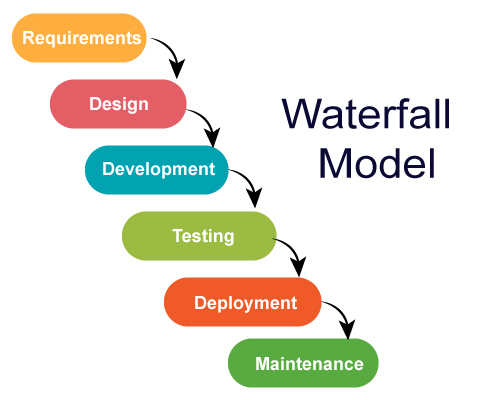
\includegraphics[width=\linewidth]{img/waterfall.png}
        \end{minipage}
        \begin{minipage}{0.3\linewidth}
            \caption{2000s敏捷开发}
            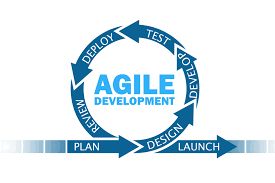
\includegraphics[width=\linewidth]{img/agile.png}
        \end{minipage}
        \begin{minipage}{0.3\linewidth}
            \caption{2010s DevOps}
            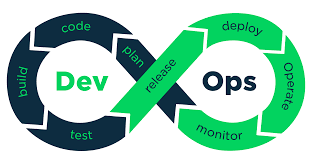
\includegraphics[width=\linewidth]{img/devops.png}
        \end{minipage}
    \end{center}
    \footnotesize{资料来源:51CTO}
\end{figure}

除此以外,企业上云也提升了Atlassian作为SaaS企业的价值,疫情带来的居家远程办公也进一步使Atlassian受益。大型企业上云重构了企业内部的沟通关系,以往利用邮件/人工/自建服务器追踪错误、维护文档移植到云上过于低效/复杂,云上的Jira、Confluence等在此时价值被企业所认知。远程办公对协作提出了更高的要求,Atlassian因此受益获得戴维斯双击。
% \begin{figure}[H]
%     \caption{软件开发越来越规范化,更倾向使用辅助工具}
%     \begin{center}
%         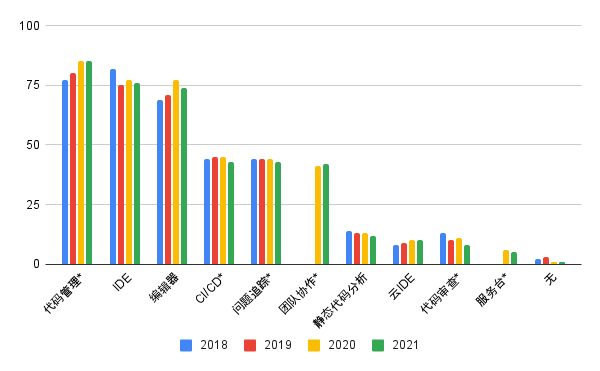
\includegraphics[width=0.9\linewidth]{img/tools.png}
%     \end{center}
%     \footnotesize{资料来源:Statista。注:标*为Atlassian覆盖的产品。}
% \end{figure}
\subsection{公司自身的\texorpdfstring{$\alpha$}——围绕团队合作打造Jira生态}
Atlassian CRO总结了其公司成长的飞轮模型\footnote{https://www.atlassian.com/blog/strategy/flywheel-effect-10-lessons},是三个组成部分构成的良性循环:吸引、参与、愉悦,即
\begin{enumerate}
    \item 通过优秀的产品吸引客户试用;
    \item 客户再试用的过程中感受到产品价值并付费;
    \item 付费的客户成为产品的推广者,将其在公司内容进行推广;
    \item 客户在使用产品的过程中发现其他产品并试用;
\end{enumerate}
\begin{figure}[H]
    \caption{Atlassian总结的成长飞轮模型}
    \begin{center}
        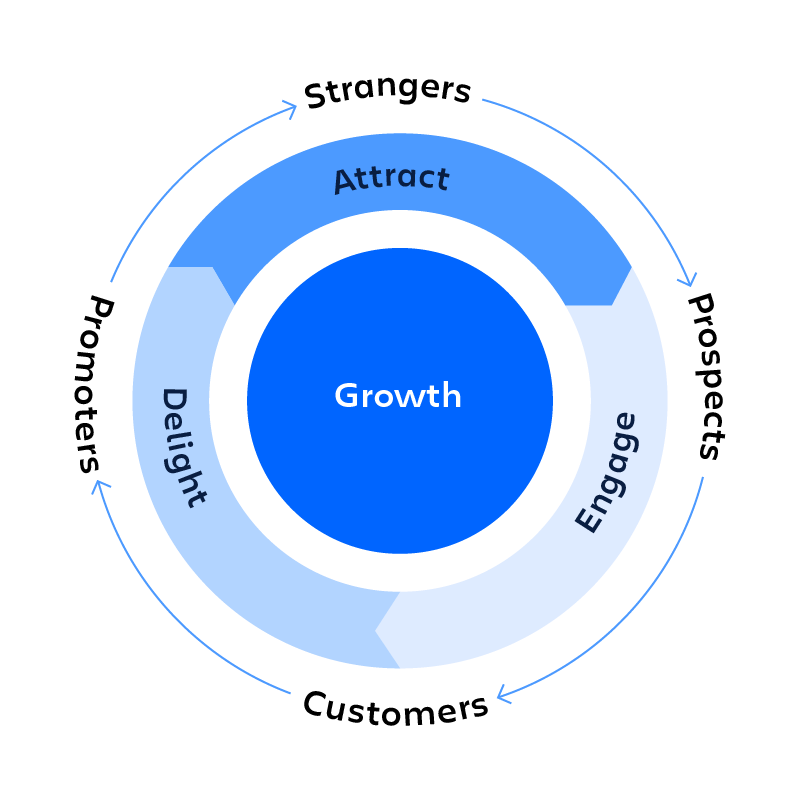
\includegraphics[width=0.8\linewidth]{img/flywheel.png}
    \end{center}
    \footnotesize{资料来源:Atlassian blog}
\end{figure}
\subsubsection{围绕核心产品Jira,专注于团队合作}
\textbf{飞轮的转动需要优秀产品的前提,Jira是一个复杂但优秀的软件}。Jira的复杂性来自于软件开发的复杂性,需要及时响应不同的需求、跟踪并分配质量参差不齐的issue、与复杂的代码有较高的集成度并能完成一定的自动化。这种复杂也给了技术人员自定义的权力,技术人员可以通过标准的或是自定义的工作流来处理软件开发中的实际问题,并获得效率上的提升。

\textbf{Atlassian专注于团队协作}。除收购的Trello外,Atlassian鲜有通用领域的产品,许多产品均是衍生自核心产品Jira的日常使用中,向外拓展进一步完善团队合作。典型例子如团队成立第二年便发布了Confluence,因为团队思考公司协作开发时需要做的所有事情,包括文档的集成。

\textbf{而对验证为无益于团队协作的产品,Atlassian会选择及时止损,并根据经验教训进行补充完善}。例如内部工作聊天软件Hipchat,Atlassian在Hipchat上复制了Jira复杂性,便于技术人员自定义但不利于一般地沟通,最终输给了Slack。Atlassian及时停止了该项目,并入股Slack在Slack中集成了Jira。

\textbf{高产品力也带动了Jira生态共荣}。Atlassian Marketplace年GMV约6亿美元\footnote{1月累计销售额达\href{https://www.atlassian.com/blog/announcements/shareholder-letter-q2fy22}{20亿},10月累计销售额达\href{https://www.linkedin.com/posts/amit-deshpande-785b3449_job-detail-atlassian-activity-6988005559119568896-mPG2?utm_source=share&utm_medium=member_desktop}{25亿}}。产品的高自定义能力吸引开发者自定义新的高效工作流并出售获利,实现生态内的共荣。
\subsubsection{免费与集成吸引潜在用户群}

\textbf{Atlassian的免费定价策略圈定了广泛的潜在客户群}。Atlassian成立之初软件公司大多依靠一次性付费许可,只有付费后才可以使用软件并且不可撤销。Atlassian则采用了免费试用的模式,这使得 Atlassian长期存续。如今Atlassian的许多产品如Jira都是对10人以下的小型团队、开源项目以及教育用途免费,吸引了广泛的用户。这些用户使用Jira等软件成为习惯时,成长后的公司或用户跳槽到的公司也会在这些用户的飞轮带动下使用 Atlassian的产品。

此外,Atlassian集成在各种编程所需的工具中,如聊天软件、IDE、代码托管网站等,进一步地扩大潜在用户群体。

\subsubsection{低成本营销带来成本优势}
\textbf{自助式销售降低了营销成本}。正如 Atlassian自己所说\footnote{\url{https://www.atlassian.com/blog/announcements/atlassian-founders-20-years-20-lessons}},软件应当被购买,而不是被出售。Atlassian 通过官网让用户自主选择产品套餐,在主页上有完全透明的价格体系,用户选择好产品类型、团队人数和部署方式后,就可以清楚地看到价格,并立即申请试用。这需要Atlassian持续降低销售中的摩擦,丰富自身文档的可用性和可达性,从而减少一对一地吸引潜在客户。

\textbf{依靠用户口碑宣传}。Atlassian 把 to B 的生意做成 to C,不仅产品是标准化 SaaS 软件,连销售方式也是如同电商一般,在用户之中的口碑是 Atlassian 最有力的武器,许多使用过Atlassian 产品的个人用户都愿意为其站台,达成飞轮效应。

\textbf{低成本的营销带来了低成本的优势}。在1Q23电话会上被问及产品的竞争优势时,管理层指出相较于其他产品, Atlassian的价格低于绝大多数替代品,较低的营销成本为有吸引力的价格打下了基础。

\subsubsection{研发驱动,鼓励创新的文化}

\textbf{Atlassian是一家研发型公司}。Atlassian研发费用率维持在45\%以上,横向对比其他SaaS公司也位于前列。高研发支出使得出品的软件大多为精品,增强用户口碑。

\textbf{Atlassian公司文化鼓励创新}。公司每年会举行hackathon ShipIt,鼓励员工和生态内的合作伙伴抽出一天时间尝试新想法并付诸实践。JSM的前身Jira 服务台便是ShipIt的产品。
\begin{figure}[H]
    \caption{Atlassian横向比较研发费用率也很高}
    \begin{center}
        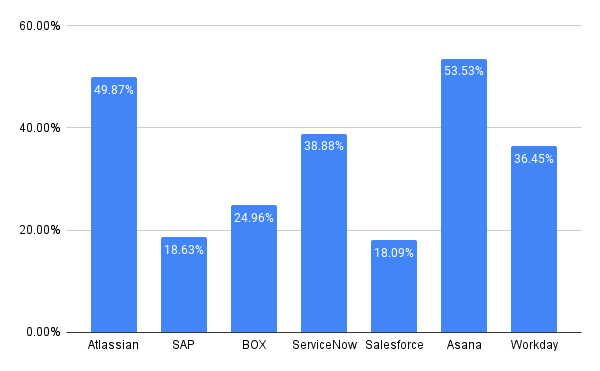
\includegraphics[width=0.9\linewidth]{img/RD.png}
    \end{center}
    \footnotesize{资料来源:Wind}
\end{figure}

\section{当前面对的困境:宏观压力、增长降速}

过去一年 Atlassian 增长动力在许多方面都受到了挑战,当前面临的困境既有外部高通胀、高利率、强竞争等因素影响,也有企业内部战略选择、产品能力有关。

\textbf{宏观逆风抑制免费用户转化率与现有用户付费意愿}。尽管云计算成为了企业必要支出,但在当前通货膨胀、能源价格上涨、美元加息影响持续,企业正减少支出以应对市场的不确定性,短期内企业在云计算上的投入相对保守,影响飞轮的转化。
\begin{figure}[H]
    \caption{宏观逆风显现,全球云计算增速放缓}
    \begin{center}
        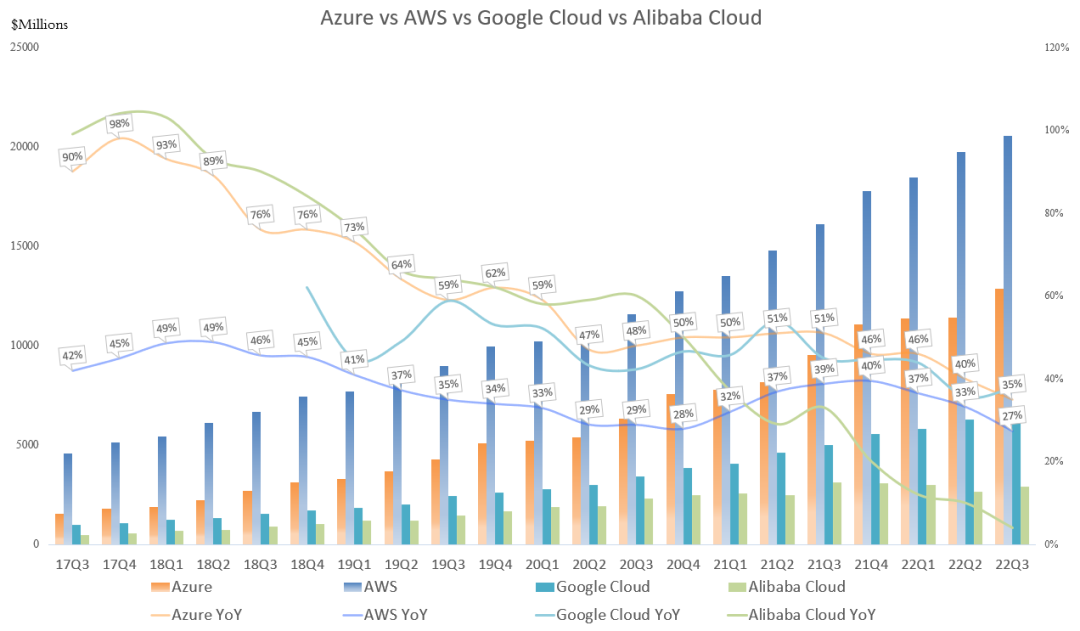
\includegraphics[width=\linewidth]{img/cloud.png}
    \end{center}
    \footnotesize{资料来源:Wind}
\end{figure}

\textbf{竞争对手的冲击}。Atlassian的竞争对手有许多大型公司,如微软的Azure Board/GitHub Enterprise/Teams等应用有广泛的用户基础,叠加其AI、云计算能力可能会形成降维打击。过去面临即时通讯领域与微软的竞争中Atlassian曾落入下风,微软等企业的扩张对 Atlassian影响有待观察。

\textbf{产品伴随网络安全风险}。利用Atlassian漏洞\footnote{\url{https://www.cvedetails.com/vulnerability-list/vendor_id-3578/Atlassian.html}}的大范围攻击可能会造成用户流失\footnote{\url{https://capital.com/atlassian-stock-forecast-team-shares-growth}},特别是Atlassian用户均为企业用户看重安全性。

\textbf{企业逆周期扩张带来短期盈利压力}。在增速放缓时选择扩张市场份额是企业的战略行为,长期看如果衰退没有超出企业预期通常可以带来好的结果。逆周期扩张短期内会使得企业在营收放缓的同时S\&M、G\&A支出扩张,尽管S\&M、G\&A支出占比相对较小,费用增速超过营收增速仍会给企业带来盈利压力。
\begin{figure}[H]
    \caption{S\&M、G\&A费用增加带来盈利压力}
    \begin{center}
        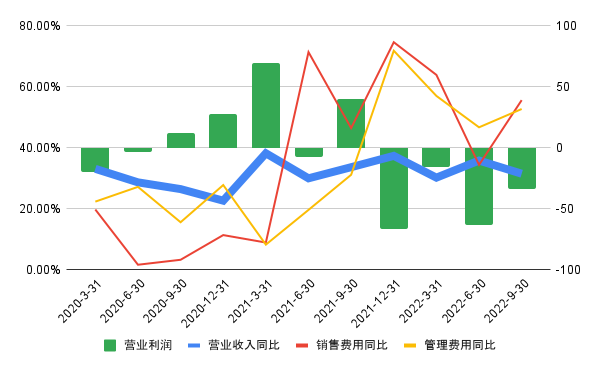
\includegraphics[width=0.8\linewidth]{img/rates.png}
    \end{center}
    \footnotesize{资料来源:Wind}
\end{figure}


\section{未来展望:短期增长承压,长期关注竞争}
基本面没有什么大问题,行业受宏观影响短时间承压但长期向好。产品粘性依旧很强,但是竞争对手的产品也在不断提升,这个是需要关注的。
\section{风险提示}
\begin{enumerate}
    \item 宏观衰退抑制企业IT支出
    \item 免费用户转化率不足
    \item 企业上云进度不及预期
    \item 新产品研发渗透不及预期造成较大的沉没成本
    \item 竞争不及对手
    \item 网络安全风险
\end{enumerate}

\end{document}
